\section{Optique géométrique et interférences}

L'\textbf{optique géométrique} (\textit{geometrical optics}) est élémentaire et
permet d'étudier les phénomènes lumineux lorsque tous les objets qui
interagissent avec la lumière ont des tailles caractéristiques grandes devant la
longueur d'onde du rayon lumineux. Nous verrons qu'elle a des limites et ne
permet donc pas d'expliquer certains phénomènes lumineux comme la diffraction ou
les interférences. Les lois générales d'optique géométrique peuvent être déduites
des équations de Maxwell et du \textbf{principe de Fermat}
(\textit{Fermat's principle}) --- la lumière se propage d'un point à un autre sur
des trajectoires telles que la durée du parcours soit stationnaire, que l'on
pourra comprendre, pour simplifier, par \emph{minimale}. Il est également
possible --- et c'est la méthode qui sera en partie choisie ici --- de poser ces
lois générales comme l'on poserait des axiomes, des expériences simples venant
les valider.\\

Ce chapitre est considéré comme un prérequis. It is not lectured in this course,
and the interference material collected in the second half is a prerequisite in
exactly the same sense.

\subsection{Principes fondamentaux}

\subsubsection{Indice de réfraction}

\begin{definition}[Indice de réfraction]
  Localement, l'\textbf{indice de réfraction} (\textit{refractive index}) $n$
  d'un milieu est le rapport de la vitesse de la lumière dans le vide $c$ sur la
  vitesse de la lumière $v$ dans le milieu considéré infini, isotrope et
  permanent :
  \[ n = \frac{c}{v}. \]
\end{definition}

L'indice caractérise en quelque sorte le ralentissement de la lumière par
rapport à sa vitesse dans le vide, $c \simeq 3\cdot 10^{8}\ \mathrm{m/s}$ : c'est
le \textbf{facteur de ralentissement} (\textit{slowing-down factor}) de la
lumière. La vitesse de la lumière dans le vide, appelée également
\textbf{célérité} (\textit{celerity}), est la vitesse maximale de la lumière :
$v \le c$. L'indice est donc toujours supérieur ou égal à 1 :

\[ n \ge 1 \quad \text{for every medium.} \]

Comme nous le verrons plus tard, l'indice dépend de la longueur d'onde du rayon
lumineux considéré.

\begin{center}
  \begin{tabular}{ll}
    \toprule
    Milieu & Indice \\
    \midrule
    vide                              & $n = 1$ \\
    air (20\textdegree C, 1 atm)      & $n = 1{,}000292$ \\
    eau                               & $n = 1{,}33$ \\
    verres                            & $n = 1{,}4$ à $1{,}9$ \\
    diamant                           & $n = 2{,}4$ \\
    germanium (semi-cond)             & $n \sim 4$ \\
    \bottomrule
  \end{tabular}
\end{center}

\subsubsection{Chemin optique d'un rayon lumineux le long d'une courbe quelconque et temps de parcours}

Suivant la valeur de l'indice de réfraction, la vitesse de la lumière varie.
Ainsi, pour une longueur \emph{physique} donnée d'un milieu traversé, le temps de
propagation ne sera pas identique. La notion de longueur physique en optique
n'est donc pas suffisante. On préférera utiliser la notion de
\textbf{chemin optique} (\textit{optical path}), qui pondère la longueur physique
par l'indice de réfraction.

\begin{definition}[Chemin optique]
  Localement, entre deux points voisins distants de $ds$, sur une courbe
  quelconque $C$, le chemin optique est défini par $dL = n\,ds$, $n$ étant
  l'indice optique du milieu au point considéré. Le chemin optique entre deux
  points $A$ et $B$ de cette courbe est par définition l'intégrale curviligne le
  long de la trajectoire considérée :
  \[ L_{\text{optique}}(AB) = \int_{AB} n\, ds. \]
  $n$ n'est ici pas forcément une constante et varie le long de $C$.
\end{definition}

Un milieu homogène, infini, permanent et isotrope est caractérisé par un indice
optique uniforme. Si on reprend l'expression du chemin optique, celle-ci devient

\[ L_{\text{optique}}(AB) = \int_{AB} n\, ds = n\, L_{\text{physique}}. \]

Le temps de parcours suivant une trajectoire de longueur $L_{\text{physique}}$
est alors

\[ t = \frac{L_{\text{physique}}}{v}
     = \frac{n\, L_{\text{physique}}}{c}
     = \frac{L_{\text{optique}}}{c}. \]

\begin{remark}
  The \emph{chemin optique} is divided by $c$, not by $v$: dividing it by $v$
  would introduce $n^{2}$. Every member holds; the last two,
  $t = n L_{\text{physique}}/c = L_{\text{optique}}/c$, show that the chemin optique is
  precisely the distance light would have covered \emph{in vacuum} in the same
  time.
\end{remark}

\subsubsection{Propagation rectiligne dans un milieu homogène, infini, permanent et isotrope}

\begin{postulate}[Propagation rectiligne (\textit{rectilinear propagation})]
  Dans un milieu homogène, l'indice $n$ est constant et la lumière se propage en
  ligne droite.
\end{postulate}

This follows directly from the expression above, with $n$ constant. Il en résulte
que $L_{\text{optique}}$ est minimal si $AB$ s'identifie à une droite. The
Fermat-stationary trajectory is therefore the straight line. Un exemple de milieu
homogène est le vide ou l'air si la température et la pression sont constantes.\\

Two experiments make the principle visible, the first with a mask in front of a
source. Les phénomènes d'ombres et de pénombres s'expliquent aisément à partir du
principe de propagation rectiligne. De même, un faisceau laser (HeNe par
exemple), matérialisé par la diffusion de particules de fumée, donne une idée de
la propagation rectiligne.

\begin{example}[Transit time over 100\,km]
  Calculer le temps de propagation de la lumière pour un chemin physique de
  $100$\,km dans l'air puis dans une fibre en verre pour des longueurs d'onde de
  $\lambda = 0{,}6\ \mu$m. Refaire ces calculs pour la longueur d'onde Télécom de
  $\lambda = 1{,}55\ \mu$m.\\

  With $L_{\text{physique}} = 10^{5}$\,m and $c \simeq 3\cdot 10^{8}$\,m/s the
  vacuum transit is $L/c = 333{,}3\ \mu$s. In air, $n = 1{,}000292$ gives
  \[ t_{\text{air}} = \frac{n L}{c} = 1{,}000292 \times 333{,}3\ \mu\mathrm{s}
     \simeq 333{,}4\ \mu\mathrm{s}, \]
  i.e.\ only about $0{,}1\ \mu$s more than in vacuum. In a glass, the table of
  indices above gives $n = 1{,}4$ to $1{,}9$; taking a representative
  $n = 1{,}5$,
  \[ t_{\text{verre}} = 1{,}5 \times 333{,}3\ \mu\mathrm{s} = 500\ \mu\mathrm{s}. \]
  The point of the second question is that $n = n(\lambda)$: the same $100$\,km
  of the same fibre is not crossed in the same time at $0{,}6\ \mu$m and at
  $1{,}55\ \mu$m, and evaluating the difference requires the dispersion curve of
  the glass, which is not tabulated here. The order of magnitude worth carrying
  away is that a fibre link costs roughly $5\ \mu$s of latency per kilometre,
  about half again the free-space figure.
\end{example}

\subsubsection{Principe d'indépendance des faisceaux lumineux}

\begin{postulate}[Indépendance des faisceaux lumineux (\textit{independence of light beams})]
  Les rayons lumineux traversant un même milieu sont indépendants les uns des
  autres.
\end{postulate}

Cela se traduit de deux façons. D'une part, dans un faisceau de rayons lumineux,
l'action sur certains rayons (arrêt, déviation, \dots) n'a aucun effet sur les
autres : l'éclairement de l'écran au-dessus du point $A$ reste inchangé quand on
intercepte une partie du faisceau, $E_1 = E_2$. D'autre part, quand deux
faisceaux se croisent, il n'y a pas d'interaction : il en est de même,
$E'_1 = E'_2$, après que l'on ait fait se croiser les faisceaux I et II.

\begin{remark}[Limits of the two preceding principles]
  Une observation très précise de la frontière séparant la lumière de l'ombre
  montre des variations d'éclairement qui ne peuvent être expliquées par les deux
  principes de propagation rectiligne et d'indépendance des rayons. Seule la
  théorie ondulatoire de la lumière permet de préciser ce phénomène
  d'éparpillement, ce qui sera vu par la suite au chapitre « diffraction ».
\end{remark}

\begin{remark}[What about interference?]
  Les interférences ne se produisent qu'en présence d'un détecteur, qui effectue
  le module au carré de la \emph{somme} des champs. Pas de détecteur, pas
  d'interférence, même quand les faisceaux se croisent. The principe
  d'indépendance des faisceaux lumineux is a statement about the fields, not
  about what a \textbf{détecteur quadratique} (\textit{square-law detector})
  reports.
\end{remark}

\subsubsection{Principe du retour inverse}

\begin{postulate}[Principe du retour inverse (\textit{inverse return})]
  Dans les milieux transparents, le trajet effectivement suivi par la lumière
  d'un point $A$ vers un point $B$ (resp.\ de $B$ vers $A$) est indépendant du
  sens de parcours.
\end{postulate}

Ce principe est valable même dans les milieux hétérogènes où le trajet est
courbe, comme nous le montrerons plus tard dans le chapitre « fibre optique ».
Une \textbf{autocollimation} réalisée avec un faisceau laser sur un miroir plan
montre la validité du principe du retour inverse. Un \textit{collimateur} est un
dispositif optique permettant d'obtenir un faisceau de rayons de lumière
parallèles à partir d'une source de lumière. Ce mot vient du latin
\textit{collimatio} (« ajuster ou viser en ligne droite »).

\subsection{Réflexion et réfraction, loi de Descartes-Snell}

\begin{definition}[Dioptre]
  Un \textbf{dioptre} (\textit{refracting interface}) est une surface séparant
  deux milieux transparents d'indices de réfraction différents, par exemple la
  surface entre l'air et l'eau.
\end{definition}

\begin{definition}[Réfraction]
  Si la lumière se propage en ligne droite dans un milieu homogène et isotrope
  (invariant par rotation), elle est déviée lors de la traversée d'un dioptre :
  c'est le phénomène de \textbf{réfraction}.
\end{definition}

\subsubsection{Lois de Descartes-Snell}

Ces lois ont été trouvées par W.~Snell en 1621 et retrouvées par R.~Descartes en
1636 --- la première mention de la loi de la réfraction a été faite par Ibn Sahl
autour de 984. Elles permettent de connaître le changement de direction, par
réflexion ou par réfraction, d'un rayon lumineux rectiligne, à la traversée d'une
surface (dioptre) séparant deux milieux homogènes. Ces lois sont au nombre de 3.

\begin{theorem}[Lois de Descartes-Snell (\textit{Descartes--Snell laws})]
  \begin{subpart}
    \item Les rayons incident, réfléchi, réfracté et la normale au point
      d'incidence à la surface du dioptre sont \textbf{coplanaires}.
    \item Le rayon réfléchi est symétrique du rayon incident par rapport à la
      normale au point d'incidence :
      \[ i = -r. \]
    \item Les sinus des angles de réfraction et d'incidence sont dans un rapport
      constant :
      \[ n \sin i = n' \sin i'. \]
  \end{subpart}
\end{theorem}

\begin{notation}
  Angles are measured from the normal to the dioptre. $n$ and $i$ are the index
  and the angle on the incidence side, $n'$ and $i'$ the index and the angle on
  the transmission side, $r$ the reflection angle. The reflection law is written
  $i = -r$ (signed angles, measured on either side of the normal), which in
  magnitude is $i = r$.
\end{notation}

\begin{figure}[h!]
  \centering
  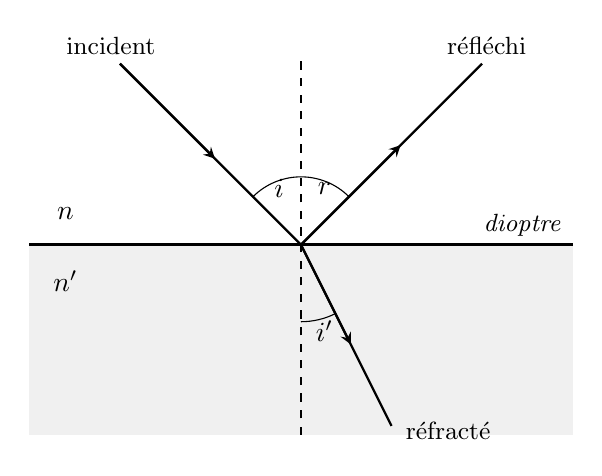
\begin{tikzpicture}[>=stealth,scale=1.15]
    \fill[gray!12] (-3.0,-2.1) rectangle (3.0,0);
    \draw[very thick] (-3.0,0) -- (3.0,0);
    \draw[dashed] (0,-2.1) -- (0,2.1);
    % incident
    \draw[thick] (-2.0,2.0) -- (0,0);
    \draw[->,thick] (-2.0,2.0) -- (-0.95,0.95);
    % reflected
    \draw[thick] (0,0) -- (2.0,2.0);
    \draw[->,thick] (0,0) -- (1.1,1.1);
    % refracted
    \draw[thick] (0,0) -- (1.0,-2.0);
    \draw[->,thick] (0,0) -- (0.55,-1.1);
    % angle arcs
    \draw (0,0.75) arc (90:135:0.75);
    \node at (-0.24,0.62) {$i$};
    \draw (0,0.75) arc (90:45:0.75);
    \node at (0.26,0.62) {$r$};
    \draw (0,-0.85) arc (270:296.5:0.85);
    \node at (0.26,-0.95) {$i'$};
    \node at (-2.6,0.35) {$n$};
    \node at (-2.6,-0.4) {$n'$};
    \node at (2.05,2.2) {\small réfléchi};
    \node at (-2.1,2.2) {\small incident};
    \node[right] at (1.05,-2.05) {\small réfracté};
    \node[rotate=0] at (2.45,0.22) {\small \textit{dioptre}};
  \end{tikzpicture}

  \smallskip
  {\small\itshape The three lois de Descartes-Snell at a dioptre: coplanarity,
  $i=-r$, $n \sin i = n' \sin i'$.}
\end{figure}

\begin{example}[The broken stick (le bâton brisé)]
  La loi de la réfraction explique pourquoi, lorsque l'on trempe une partie d'un
  bâton dans l'eau, on a l'impression que celui-ci est cassé. L'extrémité du
  bâton émet des rayons lumineux dans toutes les directions et seuls quelques
  rayons vont parvenir à notre œil. Mais ceux-ci sont réfractés et se sont
  \emph{éloignés} par rapport à la normale en changeant de milieu eau-air pour
  parvenir à l'œil. Cette réfraction n'est pas perçue par l'œil qui construit
  l'image de la partie immergée du bâton en suivant les rayons virtuels :
  l'extrémité du bâton parait donc à un autre endroit qu'il ne l'est réellement.
\end{example}

\subsubsection{Dispersion}

La vitesse de propagation de la lumière dans un milieu matériel dépend de la
longueur d'onde ($\equiv$ la couleur). Cette dépendance de $v$ avec $\lambda$
s'appelle la \textbf{dispersion chromatique} (\textit{chromatic dispersion}). Il
en est donc de même pour l'indice :

\[ v = v(\lambda), \qquad n = n(\lambda). \]

La dispersion du vide est nulle et la dispersion de l'air est négligeable. For
most purposes, then,

\[ n_{\text{vide}} = 1 \simeq n_{\text{air}}. \]

\subsubsection{Angle limite et réflexion totale}

D'après la loi de la réfraction, $n \sin i = n' \sin i'$. That is,
$\sin i' = (n/n') \sin i$. Or, on sait que $-1 \le \sin i \le 1$. The bound is on
the \emph{incidence} angle. Donc

\[ -\frac{n}{n'} \le \sin i' \le \frac{n}{n'} , \]

et suivant la valeur relative de $n$ par rapport à $n'$, deux cas se présentent.
\textbf{Réfringent} : qui cause une réfraction de la lumière. Plus le milieu est
réfringent, plus l'indice de réfraction est élevé.

\begin{subpart}
  \item $n' > n$ : le faisceau passe alors d'un milieu moins réfringent à un
    milieu plus réfringent (de l'air vers l'eau par exemple). Le rayon se
    \emph{rapproche} alors systématiquement de la normale, $i' < i$, il est donc
    toujours réfracté. Il n'y a pas d'angle limite.
  \item $n' < n$ : le faisceau passe alors d'un milieu plus réfringent à un
    milieu moins réfringent (de l'eau vers l'air). Le rayon réfracté
    s'\emph{écarte} de la normale, $i' > i$. Dans ce cas, il existe un
    \textbf{angle limite} (\textit{critical angle}) $i = i_c$ pour lequel
    l'angle de réfraction est égal à $90$\textdegree. Lorsque $i$ devient supérieur, l'expérience montre qu'il
    n'existe plus de lumière réfractée et donc transmise : il y a
    \textbf{réflexion totale} (\textit{total reflection}).
\end{subpart}

\begin{theorem}[Angle limite (ou angle critique)]
  Si $n' < n$, il existe un angle limite $i_c$,
  \[ \boxed{\ \sin i_c = \frac{n'}{n}\ } \]
  et si $i > i_c$, pas de faisceau réfracté : réflexion totale de la lumière.
\end{theorem}

\begin{figure}[h!]
  \centering
  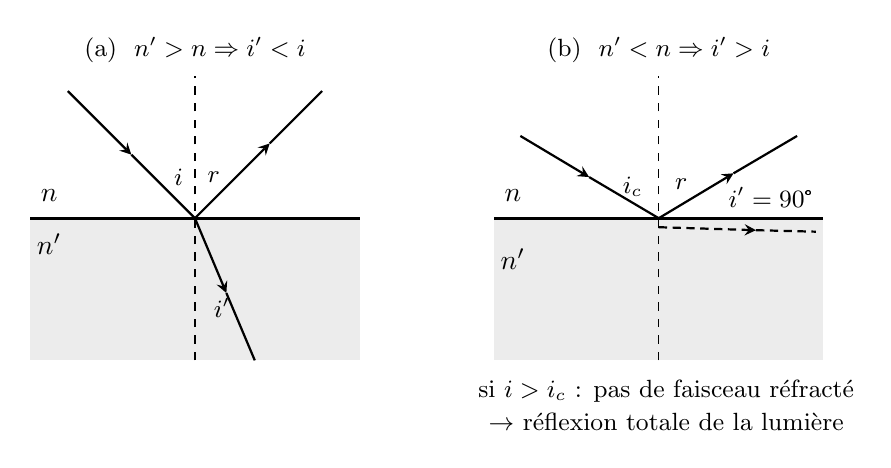
\begin{tikzpicture}[>=stealth,scale=0.95]
    % ---- panel a : n' > n ----
    \begin{scope}[shift={(0,0)}]
      \fill[gray!15] (-2.2,-1.9) rectangle (2.2,0);
      \draw[very thick] (-2.2,0) -- (2.2,0);
      \draw[dashed] (0,-1.9) -- (0,1.9);
      \draw[->,thick] (-1.7,1.7) -- (-0.85,0.85);
      \draw[thick] (-0.85,0.85) -- (0,0);
      \draw[->,thick] (0,0) -- (1.0,1.0);
      \draw[thick] (1.0,1.0) -- (1.7,1.7);
      \draw[->,thick] (0,0) -- (0.42,-1.0);
      \draw[thick] (0.42,-1.0) -- (0.8,-1.9);
      \node at (-0.22,0.55) {\small $i$};
      \node at (0.25,0.55) {\small $r$};
      \node at (0.36,-1.2) {\small $i'$};
      \node at (-1.95,0.3) {$n$};
      \node at (-1.95,-0.35) {$n'$};
      \node at (0,2.25) {\small (a)\ \ $n' > n \Rightarrow i' < i$};
    \end{scope}
    % ---- panel b : n' < n ----
    \begin{scope}[shift={(6.2,0)}]
      \fill[gray!15] (-2.2,-1.9) rectangle (2.2,0);
      \draw[very thick] (-2.2,0) -- (2.2,0);
      \draw[dashed] (0,-1.9) -- (0,1.9);
      \draw[->,thick] (-1.85,1.1) -- (-0.93,0.55);
      \draw[thick] (-0.93,0.55) -- (0,0);
      \draw[->,thick] (0,0) -- (1.0,0.6);
      \draw[thick] (1.0,0.6) -- (1.85,1.1);
      \draw[->,thick,densely dashed] (0,-0.12) -- (1.3,-0.16);
      \draw[thick,densely dashed] (1.3,-0.16) -- (2.1,-0.18);
      \node at (-0.35,0.42) {\small $i_c$};
      \node at (0.3,0.45) {\small $r$};
      \node at (1.5,0.28) {\small $i'=90$\textdegree};
      \node at (-1.95,0.3) {$n$};
      \node at (-1.95,-0.55) {$n'$};
      \node at (0,2.25) {\small (b)\ \ $n' < n \Rightarrow i' > i$};
      \node[align=center] at (0.1,-2.5)
        {\small si $i>i_c$ : pas de faisceau réfracté\\ \small $\rightarrow$ réflexion totale de la lumière};
    \end{scope}
  \end{tikzpicture}

  \smallskip
  {\small\itshape Réfraction en fonction de $n$, $n'$ et de l'angle d'incidence.
  An angle limite exists only in case (b).}
\end{figure}

Two everyday observations bracket the two cases. Chacun a déjà regardé la
surface de l'eau sur le bord d'une piscine. Il a constaté que, lorsque la surface
de l'eau est plane, quel que soit l'angle sous lequel il regarde l'eau, malgré
les reflets, il pourra voir le fond de la piscine (air to water: no angle
limite). À l'inverse, lorsque l'on fait de la plongée, si l'on essaye
de regarder la surface de l'eau avec un angle rasant, on ne voit pas du tout le
ciel, on observe au contraire un miroir parfait. Au-delà d'un certain angle
appelé angle limite, $i_c$, il y a réflexion totale.

\begin{remark}
  Comme nous le verrons plus tard, c'est l'existence d'un angle limite qui permet
  de guider la lumière dans une fibre optique par réflexion totale interne.
\end{remark}

\begin{example}[The aquarium]
  On remplit un aquarium d'eau. On éclaire la surface de l'eau avec un laser
  rouge, $\lambda = 0{,}6\ \mu$m. Take $n = 1{,}33$ for the water and
  $n_{\text{air}} = 1$.
  \begin{subpart}
    \item On oriente le laser perpendiculairement à l'eau. L'angle d'incidence se
      mesure par rapport à la normale à la surface de séparation entre les deux
      milieux (dioptre). Donc, $i = 0$\textdegree.
    \item Angle de réfraction : $\sin i' = (n/n')\sin i = 0$, so
      $i' = 0$\textdegree{} --- a ray at normal incidence is not deviated.
    \item On éclaire maintenant la surface de l'eau avec une incidence
      $i = 45$\textdegree. L'angle de réflexion est toujours identique à l'angle
      d'incidence, c'est-à-dire $r = 45$\textdegree. For the refraction,
      \[ \sin i' = \frac{n_{\text{air}}}{n_{\text{eau}}}\sin 45^{\circ}
                 = \frac{0{,}707}{1{,}33} = 0{,}532
         \quad\Longrightarrow\quad i' \simeq 32^{\circ}, \]
      the ray bending towards the normal as expected for $n' > n$.
    \item Angle limite de l'air vers l'eau. There is none: here $n' > n$, the
      refracted ray always exists; this is case (a) above and the expected answer
      is that the question has no solution.
    \item Angle limite de l'eau vers l'air :
      \[ \sin i_c = \frac{n_{\text{air}}}{n_{\text{eau}}} = \frac{1}{1{,}33}
         = 0{,}752 \quad\Longrightarrow\quad i_c \simeq 48{,}8^{\circ}. \]
  \end{subpart}
\end{example}

\subsubsection{Formules de Fresnel}

The lois de Descartes-Snell fix the \emph{directions}; the
\textbf{formules de Fresnel} (\textit{Fresnel formulas}) fix the
\emph{amplitudes}. Decomposing the incident field into a component
$E_{\parallel}$ in the plane of incidence and a component $E_{\perp}$
perpendicular to it, the amplitude reflection and transmission coefficients at a
dioptre $n_1/n_2$ are

\[ r_{\parallel} = -\frac{\tan(i-i')}{\tan(i+i')}, \qquad
   r_{\perp}     = -\frac{\sin(i-i')}{\sin(i+i')}, \]
\[ t_{\parallel} = \frac{2\cos i \sin i'}{\sin(i+i')\cos(i-i')}, \qquad
   t_{\perp}     = \frac{2\cos i \sin i'}{\sin(i+i')}. \]

\begin{remark}[Déphasage à la réflexion]
  Le \textbf{déphasage à la réflexion} (\textit{phase shift on reflection}) vaut
  $\pi$ (signe (-) de $r_{\parallel}$ et $r_{\perp}$) tant que l'on ne se trouve
  pas en réflexion totale. Dans le cas de la réflexion totale, ce déphasage est
  beaucoup plus compliqué et dépend à la fois de la polarisation et de l'angle
  d'incidence. Phénomène important dans la fibre optique.
\end{remark}

Dans le cas d'une incidence normale, on admet que le coefficient de réflexion en
amplitude sur un dioptre séparant 2 milieux d'indices $n_1$ et $n_2$ vaut

\[ r = \frac{n_2 - n_1}{n_2 + n_1}, \]

the simplified form needed for the anti-reflection coating below.

\subsection{Interférences à deux ondes}

La théorie des interférences traite de la superposition de deux ou plusieurs
champs électriques, qu'ils soient mono ou polychromatiques. Les phénomènes
ondulatoires sont décrits par une équation différentielle du second ordre
(équation de Helmholtz) et par conséquent, le \textbf{principe de superposition}
(\textit{superposition principle}) s'applique. Il en résulte qu'en tout point où
deux ou plusieurs champs optiques se superposent, l'amplitude $\v{E}$ du champ
résultant est la \emph{somme vectorielle} des amplitudes de chaque composante.

\begin{definition}[Interférences]
  Deux faisceaux \textbf{interfèrent} lorsque l'intensité résultant de la
  superposition de ces ondes n'est \emph{pas} la somme de leur intensité.
\end{definition}

Des interférences facilement observables sont celles que l'on obtient en jetant
non pas un seul mais deux cailloux dans l'eau, à deux endroits différents. Si on
regarde les rides à la surface de l'eau, il y aura des régions où les ondes se
compenseront voire s'annuleront totalement et d'autres, par contre, où les creux
et les crêtes seront accentués. Ainsi, si l'on superpose deux faisceaux
lumineux, sous certaines conditions que nous expliciterons, il est possible
d'obtenir de l'obscurité. On peut donc créer de l'obscurité avec de la lumière et
écrire alors la simple formule « lumière + lumière = obscurité ».

\subsubsection{Étude intuitive}

Soit une vibration lumineuse $E_0$ que nous séparons en deux à l'aide d'un
miroir semi-réfléchissant. Faisons parcourir à ces deux ondes deux chemins $z_1$
et $z_2$, puis re-superposons ces deux ondes. Après recombinaison, suivant les
chemins parcourus, les deux ondes peuvent se retrouver ou non en phase.

\begin{subpart}
  \item Si elles sont en phase, $\Delta\phi = 2m\pi$ avec $m$ entier, la somme
    des champs redonne le champ initial, $\v{E}_1 + \v{E}_2 = \v{E}_0$, et
    $I = I_0$ : on parle alors d'\textbf{interférences constructives}
    (\textit{constructive interference}).
  \item Si au contraire elles sont en opposition de phase, c'est que l'une des
    deux ondes a accumulé $(2m+1)\pi$ de phase en plus de l'autre. On peut alors
    écrire
    \[ \v{E}_1 + \v{E}_2
       = \v{E}_1 \underbrace{e^{2im\pi}}_{=\,1}
         \bigl(1 + \underbrace{e^{i\pi}}_{=\,-1}\bigr) = 0 . \]
    Le champ électrique s'annule. Pas de champ électrique, pas de lumière : on
    parle alors d'\textbf{interférences destructives}
    (\textit{destructive interference}), $I = 0$.
\end{subpart}

Since the phase difference is set by the path lengths, this is already a way of
\emph{coding a distance} into an intensity.

\subsubsection{Étude générale}

Considérons deux ondes lumineuses issues de la même source, monochromatiques,
polarisées rectilignement. En notation complexe, elles s'écrivent

\[ \v{E}' = E_1 e^{2i\pi\nu t}\, \v{e}_1, \qquad
   \v{E}'' = E_2 e^{2i\pi\nu t}\, \v{e}_2, \qquad
   E_1 = A e^{-i\phi_1}, \quad E_2 = A e^{-i\phi_2}, \]

où $E_1, E_2$ sont les amplitudes complexes correspondantes, $\phi_1, \phi_2$ les
phases des vibrations et $\v{e}_1, \v{e}_2$ des vecteurs unitaires portant la
direction d'oscillation du champ électrique, c'est-à-dire la direction de
polarisation. These phases are spatial. Le champ électrique résultant de la
superposition de ces deux ondes est la somme des deux champs, puisque les
équations de Maxwell auxquelles ils doivent satisfaire sont linéaires :

\[ \v{E} = \v{E}' + \v{E}'' = \bigl(E_1 \v{e}_1 + E_2 \v{e}_2\bigr) e^{2i\pi\nu t}. \]

L'intensité simplifiée de l'onde résultante sur un détecteur quadratique est

\[ I = \varepsilon_0 c |\v{E}|^{2}
     = \varepsilon_0 c \,\bigl|\v{E}' + \v{E}''\bigr|^{2}
     \propto E_1 E_1^{*} + E_2 E_2^{*}
       + \v{e}_1 \cdot \v{e}_2 \,\bigl(E_1 E_2^{*} + E_1^{*} E_2\bigr), \]

soit, après simplifications,

\[ \boxed{\ I \simeq I_1 + I_2 + 2\,(\v{e}_1\cdot\v{e}_2)\sqrt{I_1 I_2}\,
   \cos\Delta\phi \ } \]

où $\Delta\phi = \phi_2 - \phi_1$ désigne le retard de phase de l'onde 2 par
rapport à l'onde 1 (notons que l'on aurait pu prendre l'opposé car le cosinus est
pair), et $\v{e}_1 \cdot \v{e}_2$ représente le produit scalaire entre les
vecteurs unitaires portant les directions de polarisation de chaque onde. Il vaut
$1$ si les deux polarisations sont coplanaires, il est nul si elles sont
perpendiculaires.

\begin{conclusion}
  Cette équation est la formule de base de tous les problèmes d'interférences à
  deux ondes.
\end{conclusion}

\begin{remark}[Crossed polarisations]
  Lorsque les polarisations sont perpendiculaires, $\v{e}_1 \cdot \v{e}_2 = 0$ et
  $I = I_1 + I_2$ : il n'y a plus d'interférence, l'intensité totale est la
  simple addition des deux intensités.
\end{remark}

\subsubsection{Cas particulier : ondes polarisées rectilignement, coplanaires, issues d'une même source}

À partir de maintenant, les champs seront considérés comme linéairement polarisés
et \emph{de surcroît} coplanaires. Le produit scalaire vaut alors $1$ et
l'approche, théoriquement vectorielle, se réduit à un problème scalaire :

\[ I \simeq \underbrace{I_1 + I_2}_{\text{addition des intensités}}
   + \underbrace{2\sqrt{I_1 I_2}\cos\Delta\phi}_{\text{terme d'interférence}} . \]

On constate que l'intensité totale est la somme des intensités de chaque onde et
d'un \textbf{terme d'interférence} (\textit{interference term}).

\paragraph{Notion de différence de marche.} La phase de chaque onde prend la
forme

\[ \phi_1 = \phi_{\text{origine}\,1} + \phi_{\text{accumulée}\,1}, \qquad
   \phi_2 = \phi_{\text{origine}\,2} + \phi_{\text{accumulée}\,2}. \]

Les deux ondes proviennent de la même source, donc la phase à l'origine est la
même pour les deux ondes : on parle alors d'ondes \textbf{cohérentes}. La phase à
l'origine s'annule donc dans l'expression de $\Delta\phi$ et on peut pour
simplifier la considérer comme nulle,
$\phi_{\text{origine}\,1} = \phi_{\text{origine}\,2} = \phi_{\text{origine}} = 0$.
La phase accumulée dépend du chemin optique parcouru par l'onde :

\[ \phi_{\text{accumulée}\,1} = \frac{2\pi n z_1}{\lambda}, \qquad
   \phi_{\text{accumulée}\,2} = \frac{2\pi n z_2}{\lambda}, \]

où $n$ est l'indice optique du milieu et $z_1, z_2$ les distances parcourues par
chaque onde depuis leur séparation. Here $\lambda$ is the longueur d'onde in
vacuum. (Pour simplifier, on considère que les deux ondes parcourent des milieux
de même indice de réfraction $n$. Ceci n'est bien sûr pas toujours le cas.) On
peut donc en déduire l'expression du déphasage :

\[ \Delta\phi = 2\pi\frac{n(z_2 - z_1)}{\lambda} = 2\pi\frac{\delta}{\lambda},
   \qquad \boxed{\ \delta = n(z_2 - z_1)\ } \]

\begin{definition}[Différence de marche]
  La \textbf{différence de marche} (\textit{path difference}) $\delta$
  correspond à la différence de chemins optiques parcourus par les deux ondes
  depuis leur séparation jusqu'à leur recombinaison. Dans un problème
  d'interférences, tout le travail est de calculer la différence de marche entre
  les deux ondes.
\end{definition}

\paragraph{Interférence à deux ondes en lumière cohérente.} $\Delta\phi$ est
indépendante du temps, $\cos\Delta\phi$ variant dans $[-1,+1]$ :

\begin{subpart}
  \item $\Delta\phi = \pm 2m\pi \Leftrightarrow \delta = \pm m\lambda
    \Rightarrow \cos\Delta\phi = 1$ : $I$ est maximale, interférences
    constructives.
  \item $\Delta\phi = \pm(2m+1)\pi \Leftrightarrow
    \delta = \pm(2m+1)\dfrac{\lambda}{2} \Rightarrow \cos\Delta\phi = -1$ :
    $I$ est minimale, interférences destructives.
\end{subpart}

$I$ oscille entre les deux valeurs extrêmes

\[ I_{\min} = \bigl(\sqrt{I_1} - \sqrt{I_2}\bigr)^{2}, \qquad
   I_{\max} = \bigl(\sqrt{I_1} + \sqrt{I_2}\bigr)^{2}. \]

Si les amplitudes de chaque onde sont égales, c'est-à-dire $E_1 = E_2 = E_0$,
l'expression se simplifie :

\[ I(\Delta\phi) \propto 2 I_0 \bigl(1 + \cos\Delta\phi\bigr), \qquad
   I(\delta) \propto 2 I_0 \left(1 + \cos\left(2\pi\frac{\delta}{\lambda}\right)\right), \]

et le contraste des franges est alors maximum :
$I_{\max} = 4 I_0$ et $I_{\min} = 0$.

\begin{remark}
  The preceding equation $I \propto 2I_0(1+\cos\Delta\phi)$ fixes the two
  labels: the maximum is $4I_0$, reached where $\cos\Delta\phi = 1$, and the
  minimum is $0$, reached where $\cos\Delta\phi = -1$.
\end{remark}

\begin{figure}[h!]
  \centering
  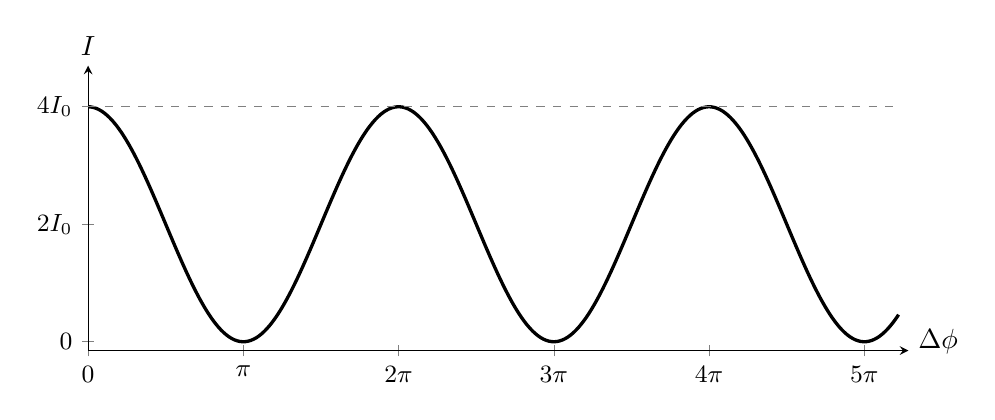
\begin{tikzpicture}
    \begin{axis}[
      width=12cm, height=5.2cm,
      axis lines=left,
      xmin=0, xmax=16.6, ymin=-0.15, ymax=4.7,
      xtick={0,3.14159,6.28319,9.42478,12.56637,15.70796},
      xticklabels={$0$,$\pi$,$2\pi$,$3\pi$,$4\pi$,$5\pi$},
      ytick={0,2,4},
      yticklabels={$0$,$2I_0$,$4I_0$},
      xlabel={$\Delta\phi$},
      ylabel={$I$},
      every axis x label/.style={at={(current axis.right of origin)},anchor=west},
      every axis y label/.style={at={(current axis.above origin)},anchor=south},
      tick label style={font=\small},
      ]
      \addplot[very thick,domain=0:16.4,samples=300,smooth]
        {2*(1+cos(deg(x)))};
      \draw[dashed,gray] (axis cs:0,4) -- (axis cs:16.4,4);
    \end{axis}
  \end{tikzpicture}

  \smallskip
  {\small\itshape Interférences à deux ondes en lumière monochromatique, si
  $I_1 = I_2 = I_0$. The same curve read against $\delta$ has its bright fringes
  at $\delta = 0, \lambda, 2\lambda, \dots$}
\end{figure}

\begin{definition}[Interfrange]
  On passe d'une frange brillante à la frange brillante suivante en faisant
  varier la différence de marche d'une longueur d'onde, soit $0{,}5\ \mu$m dans
  le jaune. On parle d'\textbf{interfrange} (\textit{fringe spacing}). The orders
  of magnitude at stake in a figure d'interférence are sub-micron.
\end{definition}

\subsection{Notion de cohérence}

Nous avons dans le cas précédent illustré la notion d'interférence à partir
d'une source unique, monochromatique, que nous avons séparée en deux puis
recombinée. Nous avons donc considéré que la phase à l'origine de l'émission
était commune aux deux ondes. Nous avons également considéré les ondes
parfaitement monochromatiques, donc avec des longueurs de \textbf{train d'onde}
(\textit{wave train}) infinies. En réalité, nous sommes à tout instant soumis à
la superposition de plusieurs ondes. Par exemple, lorsque j'allume la lumière
chez moi, je suis éclairé par les rayons issus directement de la source mais
également ceux réfléchis par les murs, le plafond. Pour autant, nous n'observons
pas de frange brillante ni sombre. Il existe donc des conditions auxquelles
doivent satisfaire deux faisceaux lumineux pour pouvoir interférer.

\subsubsection{Mécanisme d'émission par une source lumineuse}

Les ondes électromagnétiques ne sont pas émises de façon continue, mais tout se
passe comme si elles étaient émises par paquets provenant de divers atomes. Ces
atomes n'émettent pratiquement que pendant un temps limité $\tau$ qui correspond
à la durée de vie dans la théorie quantique et le coefficient d'amortissement en
théorie classique. This durée de vie is that of an excited state.\\

Si l'on attend un temps important par rapport à $\tau$, les vibrations observées
à l'instant initial auront disparu, d'autres atomes auront pris le relais, mais
les vibrations n'auront plus aucune relation avec les vibrations initiales, leur
amplitude et leur phase ayant changé. Le phénomène se reproduit un grand nombre
de fois par seconde. En d'autres termes, \emph{la phase à l'origine varie dans le
temps : elle est aléatoire}. Naturellement, cela est également vrai pour deux
vibrations émises par deux sources différentes : elles n'ont pas de relation de
phases entre elles, et la différence de phase entre les deux ondes varie
aléatoirement dans le temps.

\begin{remark}
  Tout le secret de l'émission laser réside principalement dans la mise en phase
  des différents trains d'onde successifs, comme nous le verrons plus tard dans
  le chapitre « laser ».
\end{remark}

\subsubsection{Conséquence d'une phase aléatoire dans le temps sur les interférences}

En pratique, l'intensité mesurée dépend du temps d'intégration $T_D$ du
détecteur, relié à la notion de bande passante par la formule $BP = 1/T_D$. Si la
différence de phase des deux ondes n'est pas constante dans le temps mais
aléatoire, c'est-à-dire que la lumière provient de deux sources différentes, on
ne peut pas sortir $\Delta\phi$ de la moyenne sur le temps, et l'expression de
l'intensité aurait dû s'écrire

\[ I \simeq I_1 + I_2 + 2\,(\v{e}_1\cdot\v{e}_2)\sqrt{I_1 I_2}\,
     \langle \cos\Delta\phi \rangle_{T_D},
   \qquad
   \langle \cos\Delta\phi \rangle_{T_D}
     = \frac{1}{T_D}\int_0^{T_D} \cos\Delta\phi \; dt . \]

Si de plus $\Delta\phi$ peut prendre n'importe quelle valeur de manière
aléatoire, alors

\[ \frac{1}{T_D}\int_0^{T_D} \cos\Delta\phi \; dt
   = \langle \cos\Delta\phi \rangle_{T_D} = 0
   \qquad\Longrightarrow\qquad I = I_1 + I_2 . \]

\begin{definition}[Ondes incohérentes]
  Lorsque $\Delta\phi$ est aléatoire, on dit que les ondes sont
  \textbf{incohérentes}. Il n'y a pas d'interférences : l'intensité des deux
  ondes s'ajoute simplement. When $\Delta\phi$ is fixed the ondes are
  \textbf{coherent} and $\langle\cos\Delta\phi\rangle_{T_D} = \cos\Delta\phi$.
\end{definition}

Pour réaliser des ondes cohérentes en optique, on a deux possibilités :

\begin{itemize}
  \item La \textbf{division d'amplitude} (\textit{division of amplitude}), comme
    par exemple un faisceau laser séparé en deux ou comme dans l'interféromètre
    de Michelson où la lumière est séparée par un miroir semi-réfléchissant.
  \item La \textbf{division du front d'onde} (\textit{division of wavefront})
    --- cf.\ les \textbf{trous d'Young} (\textit{Young's slits}).
\end{itemize}

\subsubsection{Notion de longueur de cohérence}

Jusqu'à présent, nous avons considéré qu'il y avait des interférences parfaites
si la source était parfaitement monochromatique (train d'onde infini
temporellement). Par interférences parfaites on veut dire que les oscillations
d'intensité $I$ lorsque la différence de marche $\delta$ augmente étaient toutes
de même amplitude. En fait, ceci n'est jamais parfaitement réalisé en pratique,
pour deux raisons : aucune source (même un laser) n'est parfaitement
monochromatique, et très peu de sources émettent des ondes planes pures.\\

Les trains d'onde ne sont pas infinis temporellement. Ceci est à l'origine d'un
\textbf{brouillage de franges} (\textit{fringe scrambling}) progressif à mesure
que la différence de marche $\delta$ augmente. En effet, les trains d'onde
n'interfèrent que s'ils se recouvrent spatialement ($\equiv$ temporellement). Au
fur et à mesure que la différence de marche augmente, le contraste diminue,
puisqu'une partie des trains d'onde ne participent plus aux interférences, ne
faisant que s'ajouter en intensité. Le contraste des franges diminue jusqu'à
disparition complète des franges.

\begin{definition}[Longueur de cohérence (\textit{coherence length})]
  Au-delà d'une certaine différence de marche dépendant de la source, il n'y a
  plus d'interférence. On appelle cette valeur de $\delta$ la
  \textbf{longueur de cohérence temporelle} de la source, $L_c$. It is the
  spatial length of a train d'onde. Les interférences seront visibles avec des
  différences de marche d'autant plus grandes que $L_c$ sera important. Les
  interférences seront donc plus facilement observables avec un laser qu'avec une
  source blanche.
\end{definition}

\begin{figure}[h!]
  \centering
  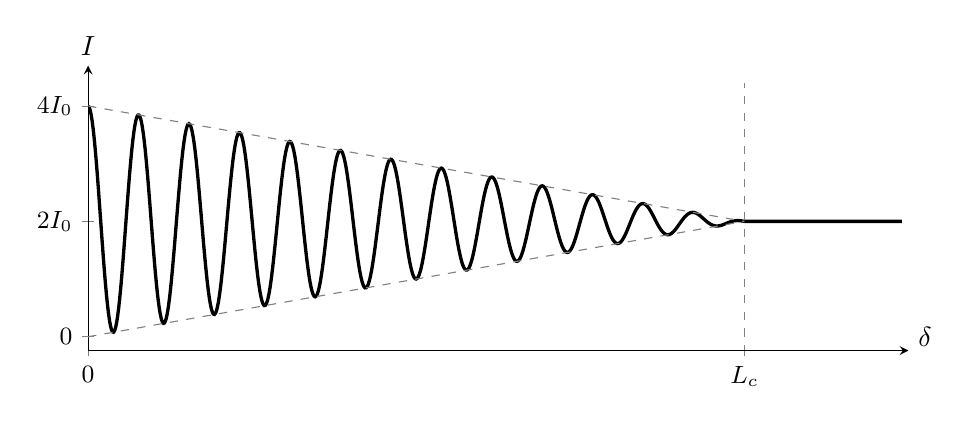
\begin{tikzpicture}
    \begin{axis}[
      width=12cm, height=5.2cm,
      axis lines=left,
      xmin=0, xmax=1.25, ymin=-0.12, ymax=2.35,
      xtick={0,1},
      xticklabels={$0$,$L_c$},
      ytick={0,1,2},
      yticklabels={$0$,$2I_0$,$4I_0$},
      xlabel={$\delta$},
      ylabel={$I$},
      every axis x label/.style={at={(current axis.right of origin)},anchor=west},
      every axis y label/.style={at={(current axis.above origin)},anchor=south},
      tick label style={font=\small},
      ]
      \addplot[very thick,domain=0:1.24,samples=800]
        {1 + max(0,1-x)*cos(deg(26*pi*x))};
      \addplot[gray,dashed,domain=0:1,samples=2]{2-x};
      \addplot[gray,dashed,domain=0:1,samples=2]{x};
      \draw[dashed,gray] (axis cs:1,0) -- (axis cs:1,2.2);
    \end{axis}
  \end{tikzpicture}

  \smallskip
  {\small\itshape Brouillage de franges: the contrast falls as $\delta$ approaches
  the longueur de cohérence $L_c$, beyond which the intensities merely add.}
\end{figure}

\subsubsection{Interférences entre deux ondes de couleurs différentes}

Lorsque la phase est aléatoire, le terme d'interférence est nul et les intensités
s'additionnent simplement. Or, le processus d'émission d'une source lumineuse
polychromatique fait qu'il n'y a \emph{pas de relation de phase entre deux
composantes de longueurs d'onde différentes}. En d'autres termes :

\begin{prop}
  Deux ondes de longueurs d'onde différentes n'interfèrent pas entre elles. Il
  suffit donc de sommer l'intensité des systèmes d'interférence créés par chaque
  longueur d'onde.
\end{prop}

Or, l'interfrange dépend de la longueur d'onde $\lambda$. The consequences in
white light are the following:

\begin{subpart}
  \item Pour $\delta = 0$, toutes les franges brillantes de chaque longueur d'onde
    sont superposées : \textbf{frange blanche} (\textit{white fringe}).
  \item Plus $\delta$ augmente, plus celles-ci se décalent spatialement. On voit
    donc apparaitre des \textbf{irisations} (\textit{iridescence}) appelées
    « \textbf{teintes de Newton} » (\textit{Newton tints}).
  \item Quand $\delta$ est trop grand, il y a brouillage des franges, on ne voit
    plus d'interférences. On parle de \textbf{blanc d'ordre supérieur}
    (\textit{white of higher order}).
\end{subpart}

\subsection{Irisation à la surface d'une nappe de pétrole}

Une nappe d'essence est une fine couche de quelques dixièmes de microns
d'épaisseur. Elle peut être assimilée à une fine lame d'indice $n$ à faces
parallèles. La lame est éclairée par une onde plane, le soleil par exemple.
Lorsque la lumière traverse ces dioptres, il se produit deux réflexions : une
première lors du passage de l'air à la couche d'indice, puis une deuxième
réflexion lors du passage de la couche d'indice à l'air. Les faisceaux émergents
sont parallèles, ils se croisent à l'infini. Là où ils se croisent, il peut se
former des interférences puisque ces deux faisceaux sont issus de la même source.

\begin{remark}
  The thickness is a few tenths of a micron, i.e.\ well under one $\mu$m: that is
  the figure that makes the physics work, since the thickness has to stay below the
  longueur de cohérence of white light.
\end{remark}

\subsubsection{Calcul de la différence de marche}

\begin{figure}[h!]
  \centering
  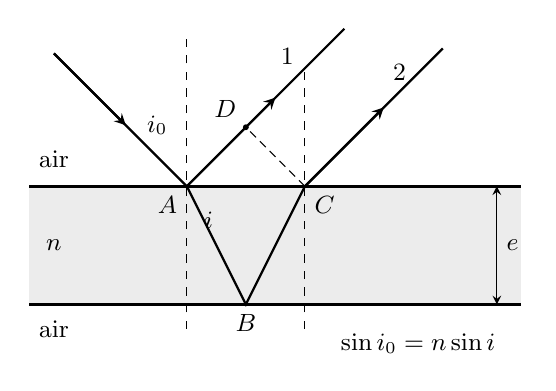
\begin{tikzpicture}[>=stealth,scale=1.25]
    % the plate
    \fill[gray!15] (-1.6,-1.2) rectangle (3.4,0);
    \draw[very thick] (-1.6,0) -- (3.4,0);
    \draw[very thick] (-1.6,-1.2) -- (3.4,-1.2);
    % normals
    \draw[dashed] (0,-1.45) -- (0,1.5);
    \draw[dashed] (1.2,-1.45) -- (1.2,1.2);
    % incident ray onto A
    \draw[thick] (-1.35,1.35) -- (0,0);
    \draw[->,thick] (-1.35,1.35) -- (-0.62,0.62);
    % reflected ray 1 at A
    \draw[thick] (0,0) -- (1.6,1.6);
    \draw[->,thick] (0,0) -- (0.9,0.9);
    \node at (1.02,1.32) {\small $1$};
    % inside: A -> B -> C
    \draw[thick] (0,0) -- (0.6,-1.2) -- (1.2,0);
    % emerging ray 2 at C
    \draw[thick] (1.2,0) -- (2.6,1.4);
    \draw[->,thick] (1.2,0) -- (2.0,0.8);
    \node at (2.16,1.16) {\small $2$};
    % D: foot of perpendicular from C onto ray 1
    \draw[densely dashed] (1.2,0) -- (0.6,0.6);
    \node[above left] at (0.6,0.6) {\small $D$};
    \fill (0.6,0.6) circle (0.03);
    % labels
    \node[below left] at (0,0) {\small $A$};
    \node[below] at (0.6,-1.2) {\small $B$};
    \node[below right] at (1.2,0) {\small $C$};
    \node at (-0.3,0.62) {\small $i_0$};
    \node at (0.22,-0.35) {\small $i$};
    \node at (-1.35,0.28) {\small air};
    \node at (-1.35,-0.6) {\small $n$};
    \node at (-1.35,-1.45) {\small air};
    \draw[<->] (3.15,0) -- (3.15,-1.2);
    \node[right] at (3.15,-0.6) {\small $e$};
    \node at (2.35,-1.6) {\small $\sin i_0 = n \sin i$};
  \end{tikzpicture}

  \smallskip
  {\small\itshape Lame d'indice $n$ à faces parallèles éclairée par une onde plane.
  Here $i$ is the angle \emph{inside} the plate. $D$ is the foot of the
  perpendicular dropped from $C$ onto ray $1$.}
\end{figure}

Un problème d'interférence commence par la résolution d'un problème géométrique.
La différence de chemin optique entre les faisceaux 1 et 2 est

\[ \Delta\ell = AB + BC - AD, \qquad
   \begin{cases}
     AB + BC = 2\,AB = 2n\dfrac{e}{\cos i}, \\[6pt]
     AD = AC \sin i_0 = 2 e \tan i \sin i_0,
   \end{cases} \]

with $i_0$ the angle of incidence in the air and $i$ the angle inside the plate,
$\sin i_0 = n \sin i$. Substituting,

\[ \Delta\ell = 2ne\left(\frac{1}{\cos i}
   - \tan i \underbrace{\frac{\sin i_0}{n}}_{\sin i}\right)
   = 2ne\,\frac{1 - \sin^{2} i}{\cos i}, \]

so that

\[ \boxed{\ \Delta\ell = \delta = 2ne\cos i \ }
   \qquad\Longrightarrow\qquad
   \boxed{\ \Delta\phi = \frac{2\pi}{\lambda}\,2ne\cos i \ } \]

\begin{remark}
  En réalité, la réflexion lame/air fait apparaître un déphasage supplémentaire
  de $\pi$ qui n'est pas pris en compte ici mais qui n'apporte rien au
  raisonnement et à la compréhension du phénomène. The formules de Fresnel above
  require it. It does swap the constructive and destructive conditions, so
  mention it if a problem asks for absolute orders.
\end{remark}

\subsubsection{Lame éclairée en lumière monochromatique}

Dans ce cas, $e$ est constant et c'est l'angle d'observation $i$ qui varie. À
l'infini, l'intensité varie suivant la formule de base des interférences à deux
ondes :

\[ I \simeq I_1 + I_2 + 2\sqrt{I_1 I_2}\,
   \cos\!\left(\frac{2\pi}{\lambda}\,2ne\cos i\right). \]

Donc, avec $m$ entier,

\[ \delta = 2ne\cos i = m\lambda
   \ \Longrightarrow\ i = \arccos\!\left(\frac{m\lambda}{2ne}\right)
   \qquad \text{(constructive)}, \]
\[ \delta = 2ne\cos i = (2m+1)\frac{\lambda}{2}
   \ \Longrightarrow\ i = \arccos\!\left(\frac{(2m+1)\lambda/2}{2ne}\right)
   \qquad \text{(destructive)}. \]

\begin{remark}
  Si on fait varier l'angle $i$, on parcourt donc les oscillations de $I$.
  Cependant, contrairement aux exemples précédemment rencontrés, la relation
  entre $\delta$ et $i$ n'est plus linéaire. Donc, sur un axe des angles
  d'incidence, les maxima de $I$ ne sont \emph{plus} également espacés.
\end{remark}

\subsubsection{Lame éclairée en lumière polychromatique : irisations}

L'angle pour lequel on obtient des interférences constructives dépend de
$\lambda$. Or, chaque figure d'interférence pour chaque longueur d'onde se somme
en intensité. Les couleurs se trouvent donc dispersées. These are the
\textit{irisations}.\\

L'observateur est fixe et observe des irisations. Lorsqu'il parcourt la surface
avec son œil, il change l'angle d'observation et donc la couleur sélectionnée. On
observe plusieurs ordres car $m$ peut valoir $1, 2, \dots$. La fonction
$\arccos(x)$ décroît lorsque $x$ augmente. Donc, \emph{quand $\lambda$
augmente, $i$ diminue}. Suivant la position de l'observateur qui regarde un
point donné de la surface, la couleur sélectionnée varie, ce qui est le cas
lorsqu'on se déplace devant une nappe irisée.

\begin{conclusion}[Why not in a bathtub]
  La réponse est directement liée à la longueur de cohérence de la lumière
  blanche, n'excédant pas quelques microns. Pour du pétrole, l'épaisseur est de
  quelques dixièmes de microns (well inside $L_c$) : les interférences sont donc
  visibles. Pour une baignoire ou une flaque d'eau, l'épaisseur est trop
  importante, bien supérieure à la longueur de cohérence d'une lumière blanche :
  les interférences sont invisibles.
\end{conclusion}

\begin{remark}
  On note sur une photo que les irisations prennent des formes irrégulières. En
  fait, cette figure d'interférence dépend de plusieurs paramètres : l'épaisseur
  de pétrole qui peut varier, les vagues qui font varier l'angle d'incidence.
  Enfin, cette démonstration est également valable pour une bulle de savon, mais
  les calculs de différence de marche sont à faire sur une sphère. C'est plus
  ardu.
\end{remark}

\subsection{Traitement anti-reflets}

Le principe des traitements anti-reflets consiste à recouvrir les dioptres de
couches transparentes minces dont l'épaisseur et l'indice sont soigneusement
déterminés, comme dans le cas précédent. Lorsque la lumière traverse un dioptre
ainsi traité, il se produit deux réflexions : une première lors du passage de
l'air à la couche anti-reflets (si la lentille est située dans l'air), puis une
deuxième réflexion lors du passage de la couche anti-reflets au verre. C'est le
fait de créer deux réflexions au lieu d'une qui va permettre d'obtenir l'effet
recherché. Si elles sont en opposition de phase, leurs effets se soustraient et
dans le cas idéal on obtient une interférence « destructive » supprimant la
réflexion. De ce fait, la lumière qui ne peut pas être réfléchie sur le dioptre
est transmise quasi intégralement par celui-ci.\\

Pour qu'une interférence destructive soit parfaite, deux conditions doivent être
réalisées. Il faut d'une part que les deux ondes aient exactement la même
amplitude et d'autre part qu'elles soient en exacte opposition de phase.

\begin{figure}[h!]
  \centering
  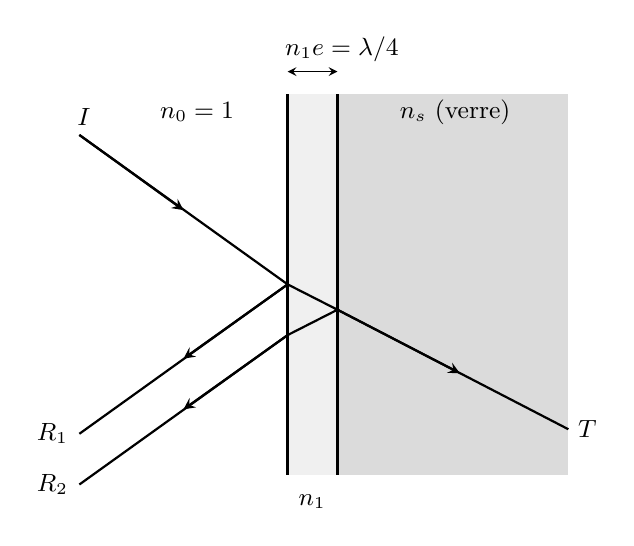
\begin{tikzpicture}[>=stealth,scale=1.15]
    \fill[gray!12] (0,-2.1) rectangle (0.55,2.1);
    \fill[gray!28] (0.55,-2.1) rectangle (3.1,2.1);
    \draw[very thick] (0,-2.1) -- (0,2.1);
    \draw[very thick] (0.55,-2.1) -- (0.55,2.1);
    % thickness marker
    \draw[<->] (0,2.35) -- (0.55,2.35);
    \node[above] at (0.6,2.35) {\small $n_1 e = \lambda/4$};
    % indices
    \node at (-1.0,1.9) {\small $n_0 = 1$};
    \node at (0.27,-2.4) {\small $n_1$};
    \node at (1.85,1.9) {\small $n_s$ (verre)};
    % incident
    \draw[thick] (-2.3,1.65) -- (0,0);
    \draw[->,thick] (-2.3,1.65) -- (-1.15,0.82);
    \node[above] at (-2.25,1.65) {\small $I$};
    % R1
    \draw[thick] (0,0) -- (-2.3,-1.65);
    \draw[->,thick] (0,0) -- (-1.15,-0.82);
    \node[left] at (-2.32,-1.65) {\small $R_1$};
    % inside
    \draw[thick] (0,0) -- (0.55,-0.28) -- (0,-0.56);
    % R2
    \draw[thick] (0,-0.56) -- (-2.3,-2.21);
    \draw[->,thick] (0,-0.56) -- (-1.15,-1.38);
    \node[left] at (-2.32,-2.21) {\small $R_2$};
    % T
    \draw[thick] (0.55,-0.28) -- (3.1,-1.6);
    \draw[->,thick] (0.55,-0.28) -- (1.9,-0.98);
    \node[right] at (3.1,-1.6) {\small $T$};
  \end{tikzpicture}

  \smallskip
  {\small\itshape Double réflexion obtenue avec une lame quart d'onde. $R_1$ and
  $R_2$ are made equal in amplitude and
  opposite in phase, so the reflection cancels and everything goes into $T$.}
\end{figure}

\paragraph{Même amplitude.} La réflexion sur un dioptre dépend directement de la
différence des indices de réfraction des deux milieux ; dans le cas d'une
incidence normale, on admet que le coefficient de réflexion en amplitude sur un
dioptre séparant 2 milieux d'indices $n_1$ et $n_2$ vaut

\[ r = \frac{n_2 - n_1}{n_2 + n_1}, \]

soit, pour une couche anti-reflet composée de 2 dioptres air/anti-reflet et
anti-reflet/verre,

\[ r_{\text{air}/\text{anti-reflet}}
     = \frac{n_{\text{anti-reflet}} - 1}{n_{\text{anti-reflet}} + 1},
   \qquad
   r_{\text{anti-reflet}/\text{verre}}
     = \frac{n_{\text{verre}} - n_{\text{anti-reflet}}}
            {n_{\text{verre}} + n_{\text{anti-reflet}}} . \]

Setting $r_{\text{air}/\text{anti-reflet}} = r_{\text{anti-reflet}/\text{verre}}$,
on montre facilement que la couche anti-reflets doit posséder un indice

\[ \boxed{\ n_{\text{anti-reflet}} = \sqrt{n_{\text{verre}}}\ } \]

\begin{example}
  Avec un verre d'indice $1{,}69$, il faut une couche d'indice $1{,}3$ pour
  réaliser l'égalité des amplitudes.
\end{example}

\paragraph{Opposition de phase.} La lumière réfléchie sur le second dioptre doit
être décalée d'une demi-longueur d'onde par rapport à celle que renvoie le
premier. La couche est traversée deux fois par la seconde onde réfléchie. With
$\delta = 2ne$, then,

\[ \Delta\varphi = \frac{2\pi \cdot 2ne}{\lambda} = m\pi
   \qquad\Longrightarrow\qquad
   \boxed{\ ne = m\,\frac{\lambda}{4}\ } \]

with $m$ odd for the destructive case: the first solution is the
\textbf{lame quart d'onde} (\textit{quarter-wave layer}), of optical thickness
$ne = \lambda/4$, i.e.\ a quarter of a longueur
d'onde \emph{measured inside the coating}.

\begin{remark}[Limits of a single layer]
  En incidence normale, la correction fournie par le traitement n'est en principe
  valable que pour une seule longueur d'onde. Si l'incidence de la lumière n'est
  pas normale au dioptre, le chemin optique se trouve allongé et la correction
  fonctionne encore mais pour une longueur d'onde un peu plus grande, donc pour un
  rayonnement décalé vers le rouge. En pratique, l'amélioration concerne presque
  tout le spectre visible, mais il n'est pas possible avec une seule épaisseur de
  traitement d'obtenir une interférence parfaitement destructive pour toutes les
  longueurs d'onde et pour tous les angles d'incidence. Il faut donc savoir en
  fonction de quelle longueur d'onde, c'est-à-dire en fonction de quelle couleur,
  cette épaisseur sera choisie. Les lentilles qui portent un traitement
  monocouche ont donc forcément un aspect coloré. La plupart du temps elles
  semblent bleutées, ce qui signifie que l'on a privilégié l'absence de réflexion
  de la couleur complémentaire, c'est-à-dire le jaune, qui est la couleur la plus
  éblouissante, qui du coup sera davantage transmis. Les traitements multicouches
  évitent la réflexion de deux ou plusieurs longueurs d'onde différentes ; les
  lentilles apparaissent alors beaucoup moins teintées que dans le cas d'un
  traitement monocouche. Cependant, le traitement mono-couche est bon marché, donc
  accessible au grand public sur les verres de lunettes de vue.
\end{remark}

\begin{conclusion}[What the course expects from this chapter]
  Comprendre la notion de chemin optique ; savoir appliquer les lois de la
  réflexion et de la réfraction ; savoir calculer l'angle limite de réflexion
  totale ; savoir calculer et représenter la figure d'interférence entre deux
  ondes planes cohérentes ; savoir calculer une longueur de cohérence ; savoir
  déterminer les conditions d'obtention d'interférences ; et savoir expliquer et
  calculer les positions des irisations sur une nappe de pétrole.
\end{conclusion}
